\chapter{ТФКП}

\section{Серия полезных результатов}

\subsection{Теорема Коши для прямоугольного треугольника}

\begin{figure}[!h]
	\centering
	\begin{subfigure}{0.4\textwidth}
		\centering
		\begin{tikzpicture}[>=Stealth]
			\draw (1, 1) -- (3, 3) node[right] {$ C $};
			\draw (1, 1) -- (3, 1) node[right] {$ B $};
			\draw (3, 1) -- (3, 3);
			\draw (1, 1) node[below] {$ A $};

			\draw (2, 1) node[below] {$ K $};
			\draw (3, 2) node[right] {$ E $};
			\draw (2, 2) node[left] {$ D $};
			\draw (2, 1) -- (2, 2) -- (3, 2);

			\draw (1.75, 1.25) node {$ \vartriangle_2 $};
			\draw (2.75, 2.25) node {$ \vartriangle_1 $};
		\end{tikzpicture}
		\caption{Прямоугольный треугольник}
		\label{pic:1a}
	\end{subfigure}
	\begin{subfigure}{0.4\textwidth}
		\centering
		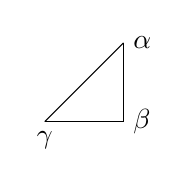
\begin{tikzpicture}
			\draw (0, 0) -- (1, 1) node[right] {$ \alpha $};
			\draw (0, 0) -- (1, 0) node[right] {$ \beta $};
			\draw (1, 0) -- (1, 1);
			\draw (0, 0) node[below] {$ \gamma $};
		\end{tikzpicture}
		\caption{}
		\label{pic:1b}
	\end{subfigure}
\end{figure}

\begin{theorem}
	Рассматриваем треугольник $ ABC $ (\autoref{pic:1a}).
	$$ f \in \mc A(G), \qquad A = a + pi, \quad B = b + pi, \quad c = b + qi, \qquad a < b, \quad p < q, \qquad \vartriangle ABC \sub G $$
	$$ I \define \cint[z]{\curvedir{\partial \vartriangle} ABC}{f(z)} = 0 $$
\end{theorem}

\begin{proof}
	Рассмотрим точки:
	$$ D = \frac{a + b}2 + i \frac{p + q}2, \qquad K = \frac{a + b}2 + pi, \qquad E = b + i \frac{p + q}2 $$
	$$ \cint[z]{\curvedir{\partial \vartriangle} ABC}{f(z)} = \int\limits_{\curvedir{\partial \Box}} + \int\limits_{\curvedir{\partial \vartriangle_1}} + \int\limits_{\curvedir{\partial \vartriangle_2}} $$
	$$ \int\limits_{\overrightarrow{ED}} + \int\limits_{\overrightarrow{DE}} = 0, \qquad \int\limits_{\overrightarrow{DK}} + \int\limits_{\overrightarrow{KD}} = 0 $$
	К каждому из треугольников можно применить такое же рассуждение, а к прямоугольникам "--- теорему Коши для прямоугольника. Получаем
	\begin{equ}1
		I = \sum_{k = 1}^{2^n} I_{n_k}
	\end{equ}
	\begin{equ}2
		I_{n_k} = \cint[z]{\curvedir{\partial \vartriangle_{n_k}}}{f(z)}
	\end{equ}
	Рассмотрим какой-то из шагов (треугольник обозначим $ \alpha\beta\gamma $, \autoref{pic:1b}):
	$$ \cint[z]{\curvedir{\partial \vartriangle}\alpha\beta\gamma}{f(z)} = \cint[z]{\curvedir{\partial\vartriangle}\alpha\beta\gamma}{f(z) - f(\alpha)} + f(\alpha) \cint[z]{\curvedir{\partial\vartriangle}\alpha\beta\gamma}1 $$
	Второй интеграл равен 0 (по св-ву 5 криволинейных интегралов). Значит, это равно
	\begin{equ}3
		\cint[z]{\curvedir{\partial\vartriangle}\alpha\beta\gamma}{f(z) - f(\alpha)}
	\end{equ}
	По св-ву 7 криволинейных интегралов, это означает, что
	\begin{equ}4
		\bigg| \cint[z]{\curvedir{\partial\vartriangle}\alpha\beta\gamma}{f(z)} \bigg| \le \acint{\partial\vartriangle\alpha\beta\gamma}{|f(z) - f(\alpha)|}
	\end{equ}
	Применим теорему Кантора:
	\begin{equ}5
		\forall \veps > 0 \quad \exist \delta > 0 : \quad \forall \alpha \in [A, C], \quad z \in \partial \vartriangle \alpha\beta\gamma \quad |f(z) - f(\alpha)| < \veps
	\end{equ}
	Выберем $ n $ так, что
	$$ z^{-n} \cdot |C - A| < \delta $$
	Тогда
	\begin{equ}7
		\eref4, \eref5 \implies \acint{\partial \vartriangle\alpha\beta\gamma}{|f(z) - f(\alpha)|} < \veps \acint{\partial\vartriangle\alpha\beta\gamma}{} \underset{\text{из геом. сообр.}}< 3\veps |\gamma - \alpha| = 3\veps \cdot |C - A| \cdot 2^{-n}
	\end{equ}
	\begin{equ}8
		\underimp{\eref4} \forall k \quad |I_{n_k}| < 3 \veps |C - A| \cdot 2^{-n}
	\end{equ}
	\begin{equ}9
		\underimp{\eref1} |I| \le \sum_{k = 1}^{2^n}|I_{n_k} < 3\veps |C - A| \cdot 2^{-n} \cdot 2^n = 3 \veps |C - A|
	\end{equ}
	$$ \implies |I| = 0 $$
\end{proof}

Если треугольник перевернуть относительно оси ординат, результат не изменится.

\begin{remark}
	Аналитичность $ f $ использовалась для прямоугольника.
\end{remark}

\subsection{Теорема Коши для треугольника}

\begin{figure}[!h]
	\centering
	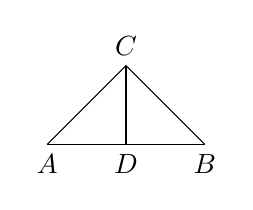
\begin{tikzpicture}
		\draw (0, 0) -- (2, 0) node[below] {$ B $};
		\draw (0, 0) -- (1, 1) node[above] {$ C $};
		\draw (1, 1) -- (1, 0) node[below] {$ D $};
		\draw (0, 0) node[below] {$ A $};
		\draw (2, 0) -- (1, 1);
	\end{tikzpicture}
	\caption{}
	\label{pic:2}
\end{figure}

\begin{theorem}
	Рассматриваем треугольник $ ABC $ (\autoref{pic:2})
	$$ A = a + pi, \quad B = b + pi, \quad C = d + qi, \qquad a < d < l, \qquad q > p $$
	$$ \underbrace{\int\limits_{\curvedir{\partial \vartriangle}ADC}}_0 + \underbrace{\int\limits_{\curvedir{\partial\vartriangle}DBC}}_0 = \int\limits_{\curvedir{\partial\vartriangle}ABC} $$
\end{theorem}

\begin{figure}[!ht]
	\centering
	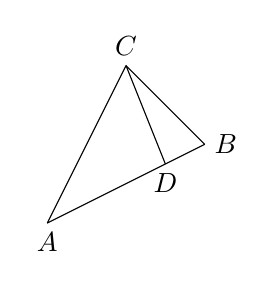
\begin{tikzpicture}
		\draw (0, 0) node[below] {$ A $};
		\draw (0, 0) -- (2, 1) node[right] {$ B $};
		\draw (0, 0) -- (1, 2) node[above] {$ C $};
		\draw (1, 2) -- (1.5, 0.75) node[below] {$ D $};
		\draw (1, 2) -- (2, 1);
	\end{tikzpicture}
	\caption{}
	\label{pic:3}
\end{figure}

\begin{theorem}
	Рассматриваем треугольник $ ABC $ (\autoref{pic:3}). Считаем, что наибольшая сторона "--- это $ AB $.

	Возьмём $ \theta $ так, что $ e^{i\theta} \cdot \vartriangle ABC $ повёрнут ``правильно''.
	$$ f_\theta(z) \define f(e^{-i\theta}z), \qquad f_\theta \in A(G_\theta) $$
	Получаем треугольник $ A_1B_1C_1 $ из предыдущей теоремы.

	Дальше пользуемся свойством 8 криволинейных интегралов.
\end{theorem}

\subsection{Теорема Коши для конечносвязной многоугольной области}

\begin{definition}
	\it{Многоугольником} будем называть замкнутую кривую $ \Gamma : [a, b] \to \Co $, устроенную следующим образом:
	$$ n \ge 2, \qquad a = c_0 < c_1 < \dots < c_n < c_{n + 1} = b $$
	$$ \forall t \in [c_k, c_{k + 1}] \quad \Gamma(t) = \Gamma(c_k) \cdot \frac{c_{k + 1} - t}{c_{k + 1} - c_k} + \Gamma(c_{k + 1}) \cdot \frac{t - c_k}{c_{k + 1} - c_k} $$

	Точки $ \Gamma(c_k) $ будем называть \it{вершинами} многоугольника.
\end{definition}

\begin{definition}
	\it{Многоугольной областью} будем называть область, граница которой является многоугольником.
\end{definition}

\begin{definition}
	\it{Конечносвязной многоугольной областью} будем называть область, граница которой состоит из конечного объединения многоугольников.
\end{definition}

\begin{theorem}
	Имеется некая конечносвязная многоугольная область $ D $, ограниченная многоугольниками $ \Gamma_1, \dots, \Gamma_k $.
	$$ \partial D = \bigcup_{\nu = 1}^k \Gamma_\nu $$
	Пусть есть область $ G $ такая, что $ G \supset \ol D $ и функция $ f \in \mc A(G) $. Рассмотрим
	$$ \curvedir \partial D = \bigcup_{\nu = 1}^k \curvedir \Gamma_\nu, $$
	при этом, каждая кривая $ \Gamma_\nu $ положительно ориентированна относительно области $ D $.
	$$ \implies \cint[z]{\curvedir\partial D}{f(z)} = 0 $$
\end{theorem}

\begin{proof}
	Применим теорему о триангуляции конечносвязной многоугольной области:
	$$ \exist \seq[N]{\Delta_k}k, \quad \Delta_k \text{ "--- откр.: } \qquad
	\begin{cases}
		\Delta_k \cap \Delta_l = \O, \quad k \ne l \\
		\ol\Delta_k \cap \ol\Delta_l =
		\begin{cases}
			\O \\
			\text{общая вершина} \\
			\text{общая сторона}
		\end{cases} \\
		\bigcup_{k = 1}^N \ol \Delta_k = \ol D
	\end{cases} $$
	Рассмотрим
	$$ \sum_{k = 1}^N \cint[z]{\curvedir{\partial\Delta}_k}{f(z)} $$
	Каждый из них предстаим в виде суммы интегралов по трём сторонам. В результате:
	\begin{enumerate}
		\item каждый внутренний отрезок мы пройдём дважды в разных направлениях;
		\item все ``внутренние'' границы (многоугольники) проходятся полностью в отрицательном (относительно самого многоугольника) направлении;
		\item остаётся только ``внешняя'' граница.
	\end{enumerate}
	$$ \sum = 0 $$
\end{proof}
